%%
%% This is file `sample-sigplan.tex',
%% generated with the docstrip utility.
%%
%% The original source files were:
%%
%% samples.dtx  (with options: `sigplan')
%% 
%% IMPORTANT NOTICE:
%% 
%% For the copyright see the source file.
%% 
%% Any modified versions of this file must be renamed
%% with new filenames distinct from sample-sigplan.tex.
%% 
%% For distribution of the original source see the terms
%% for copying and modification in the file samples.dtx.
%% 
%% This generated file may be distributed as long as the
%% original source files, as listed above, are part of the
%% same distribution. (The sources need not necessarily be
%% in the same archive or directory.)
%%
%% Commands for TeXCount
%TC:macro \cite [option:text,text]
%TC:macro \citep [option:text,text]
%TC:macro \citet [option:text,text]
%TC:envir table 0 1
%TC:envir table* 0 1
%TC:envir tabular [ignore] word
%TC:envir displaymath 0 word
%TC:envir math 0 word
%TC:envir comment 0 0
%%
%%
%% The first command in your LaTeX source must be the \documentclass command.
\documentclass[sigplan,screen]{acmart}
%% NOTE that a single column version is required for 
%% submission and peer review. This can be done by changing
%% the \doucmentclass[...]{acmart} in this template to 
%% \documentclass[manuscript,screen,review]{acmart}
%% 
%% To ensure 100% compatibility, please check the white list of
%% approved LaTeX packages to be used with the Master Article Template at
%% https://www.acm.org/publications/taps/whitelist-of-latex-packages 
%% before creating your document. The white list page provides 
%% information on how to submit additional LaTeX packages for 
%% review and adoption.
%% Fonts used in the template cannot be substituted; margin 
%% adjustments are not allowed.
%%
%% \BibTeX command to typeset BibTeX logo in the docs
\AtBeginDocument{%
  \providecommand\BibTeX{{%
    \normalfont B\kern-0.5em{\scshape i\kern-0.25em b}\kern-0.8em\TeX}}}

%% Rights management information.  This information is sent to you
%% when you complete the rights form.  These commands have SAMPLE
%% values in them; it is your responsibility as an author to replace
%% the commands and values with those provided to you when you
%% complete the rights form.
%\setcopyright{acmcopyright}
%\copyrightyear{2018}
%\acmYear{2018}
%\acmDOI{XXXXXXX.XXXXXXX}

%% These commands are for a PROCEEDINGS abstract or paper.
%\acmConference[Conference acronym 'XX]{Make sure to enter the correct
 % conference title from your rights confirmation emai}{June 03--05,
 % 2018}{Woodstock, NY}
%
%  Uncomment \acmBooktitle if th title of the proceedings is different
%  from ``Proceedings of ...''!
%
%\acmBooktitle{Woodstock '18: ACM Symposium on Neural Gaze Detection,
%  June 03--05, 2018, Woodstock, NY} 
%\acmPrice{15.00}
%\acmISBN{978-1-4503-XXXX-X/18/06}

%%
%% For managing citations, it is recommended to use bibliography
%% files in BibTeX format.
%%
%% You can then either use BibTeX with the ACM-Reference-Format style,
%% or BibLaTeX with the acmnumeric or acmauthoryear sytles, that include
%% support for advanced citation of software artefact from the
%% biblatex-software package, also separately available on CTAN.
%%
%% Look at the sample-*-biblatex.tex files for templates showcasing
%% the biblatex styles.
%%

%%
%% The majority of ACM publications use numbered citations and
%% references.  The command \citestyle{authoryear} switches to the
%% "author year" style.
%%
%% If you are preparing content for an event
%% sponsored by ACM SIGGRAPH, you must use the "author year" style of
%% citations and references.
%% Uncommenting
%% the next command will enable that style.
%%\citestyle{acmauthoryear}
\usepackage{graphicx}
\usepackage{float}
\usepackage{lipsum}
%%
%% end of the preamble, start of the body of the document source.
\begin{document}

%%
%% The "title" command has an optional parameter,
%% allowing the author to define a "short title" to be used in page headers.
\title{Event Processing Project SoSe 2022}

%%
%% The "author" command and its associated commands are used to define
%% the authors and their affiliations.
%% Of note is the shared affiliation of the first two authors, and the
%% "authornote" and "authornotemark" commands
%% used to denote shared contribution to the research.
\author{Ahmet Turkmen}


%%
%% By default, the full list of authors will be used in the page
%% headers. Often, this list is too long, and will overlap
%% other information printed in the page headers. This command allows
%% the author to define a more concise list
%% of authors' names for this purpose.
\renewcommand{\shortauthors}{Ahmet Turkmen}

%%
%% The abstract is a short summary of the work to be presented in the
%% article.
\begin{abstract}
In this paper, demonstration of event processing on Kafka + KSQL streaming platform will be considered and discussed. The input data is around 356 MB and it is structured data. 
Go programming language is used to parse and publish data to Kafka instances. Kafka + KSQL environment is set with official Docker-compose file from Github.
\end{abstract}

\maketitle

\section{Streaming Messages}

In order to stream messages to Kafka cluster, there is a need of a producer which will read and send all data to Kafka cluster. The streaming part, the producer,  of the project completed with Go programming language. 
The program creates the topic on Kafka cluster and pushes events on the given file directly to Kafka cluster. 

\subsection{Kafka Setup}
Initially, Confluent cloud\cite{confluent-cloud} trial version is used, however due to unreliable network connection on producer side and high latency on Cloud side, this approach is dismissed. 
The main idea became to setup Kafka cluster along with ksqldb. It can be achieved by simple Docker Compose file provided by confluent repository on Github\cite{cp-all-in-one}
Provided "docker-compose.yaml" file contains all required services (Zookeeper, ksqldb, ksqldb-ci, control-center, kafka and more) and additionally a web interface to easy access to topics and streams. Running instances can be observed through given Figure 1. 
\begin{figure}[H]
    \centerline{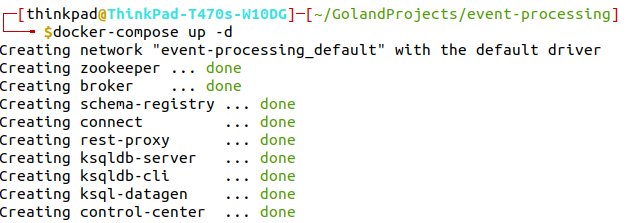
\includegraphics[scale=.4]{assets/running-docker-instances.png}}
    \caption{Running Docker Instances}
    \label{fig}
\end{figure}
Once all the containers are in running state, now streaming messages can start through Go program. 
\subsection{Stream Events}
The source of the events is a file which needs to be processed with a producer. Producer will read through the file and push them to Kafka cluster under given topic name. Figure 2 represents the source code which is responsible to stream data to created topic. 
\begin{figure}[H]
    \centerline{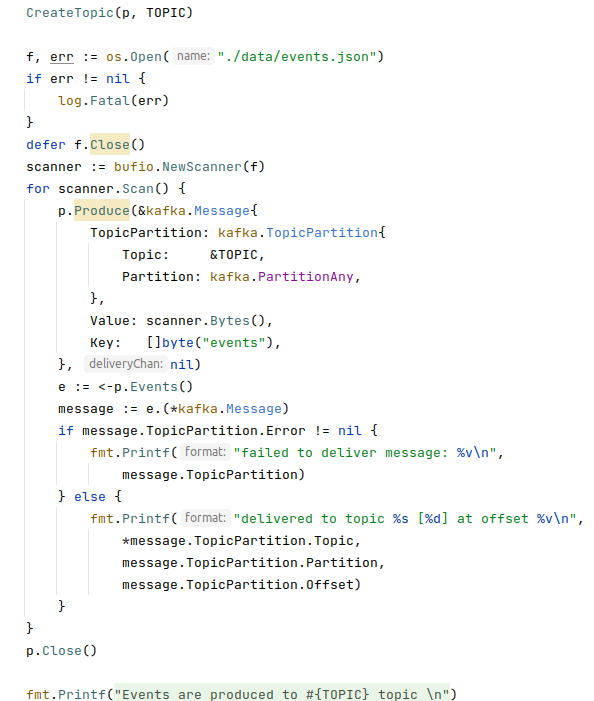
\includegraphics[scale=.4]{assets/producer-code.png}}
    \caption{Source code for streaming messages}
    \label{fig}
\end{figure}
The given events source file is scanned and pushed to topic with help of channels in Go programming language shown in Figure 2. The full source code of the project is accessible on Github\footnote{https://github.com/mrtrkmn/kafka-event-processing}

\section{Filtering}

Creating filters are done through ksqlDB, it is purpose built-in for stream processing applications\footnote{https://ksqldb.io/}. As events stream to a topic, it is possible to filter and stream filtered events to another topic based on conditions defined in the query. It is achievable through ksqlDB query in Kafka. 
In order to filter messages received from a producer, a stream needs to set, it can be done with clarifying incoming message skeleton with fields\cite{create-stream}. 
\begin{figure}[H]
    \centerline{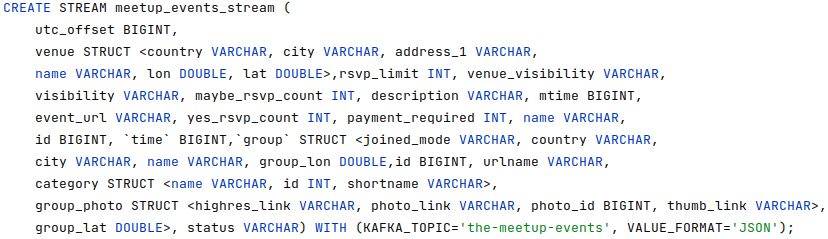
\includegraphics[scale=.3]{assets/create_stream_meetups.png}}
    \caption{Creating a stream from a topic }
    \label{fig}
\end{figure}
The query on Figure 3, creates a stream from a Kafka topic which is fed by a producer. As 
"\textt{the-meetup-events}" topic fed by producer, stream  "\textt{meetup\_events\_stream}" consumes messages from the topic. The streams enables data to analyze, manipulate, transform and filter incoming messages from given topic. 
\subsection{Country filtering}
Kafka streams are straightforward to filter, in Figure 4, incoming messages filtered based on country information they include. 
\begin{figure}[H]
    \centerline{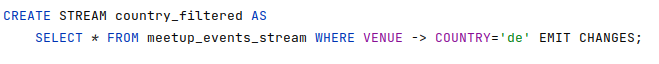
\includegraphics[scale=.3]{assets/filter_country_stream.png}}
    \caption{Filter country from a stream }
    \label{fig}
\end{figure}

New stream called \textt{country\_filtered} is created and it is saved as persistent query in ksqlDB. Persistent queries run and listen given topic to consume in background. 
\subsection{City Filtering}
In order to narrow down the search to Munich or München, two different streams are created from "\textt{meetup\_events\_stream}" stream as source. 
\begin{figure}[H]
    \centerline{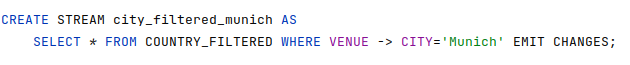
\includegraphics[scale=.3]{assets/filter_munich_stream.png}}
    \caption{Filter "Munich" city  }
    \label{fig}
\end{figure}

\begin{figure}[H]
    \centerline{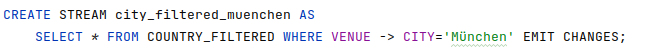
\includegraphics[scale=.3]{assets/filter_munchen_stream.png}}
    \caption{Filter "München" city }
    \label{fig}
\end{figure}

Both streams, "\textt{city\_filtered\_munich}" and "\textt{city\_filtered\_muenchen}" are consuming messages by filtering from "\textt{country\_filtered}" stream. Overall stream flow of different stream connections is shown in Figure 7. 

\begin{figure}[H]
    \centerline{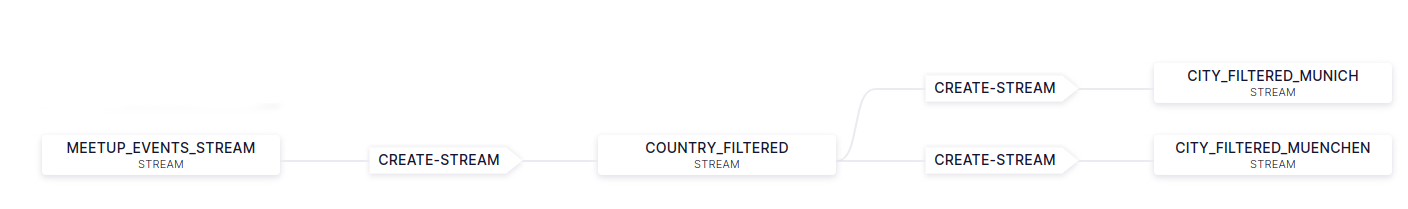
\includegraphics[scale=.2]{assets/stream_flow.png}}
    \caption{Overall stream flow  }
    \label{fig}
\end{figure}



\section{Conclusion}
In this project, Kafka + ksqldb are used as main environment, provided events file processed with created producer. The messages are filtered with help of streams on ksqlDB. However, the environment used in this project is not fault tolerant, since replication count is limited to one due to local instance. Even though number of partitions is not limited to one, it is not fault tolerant. Since a problem on the instance may cause to lost all data due to replication count being one. Throughput, latency graphs along with topics view included in Appendix. The end to end average latency is higher at the beginning and decreases to a point where it continues linear. The latency can be minimized with batch processing of events however, it has not been implemented in this experiment. The throughput of the environment is affected by system's capabilities (CPU power) and processing method of the events. 




% add bibliography
\bibliographystyle{ACM-Reference-Format}
\bibliography{bibliography}
\onecolumn
\newpage


\begin{Huge}
Appendix
\end{Huge}


\section{Overview of the cluster}
\begin{figure}[H]
    \centerline{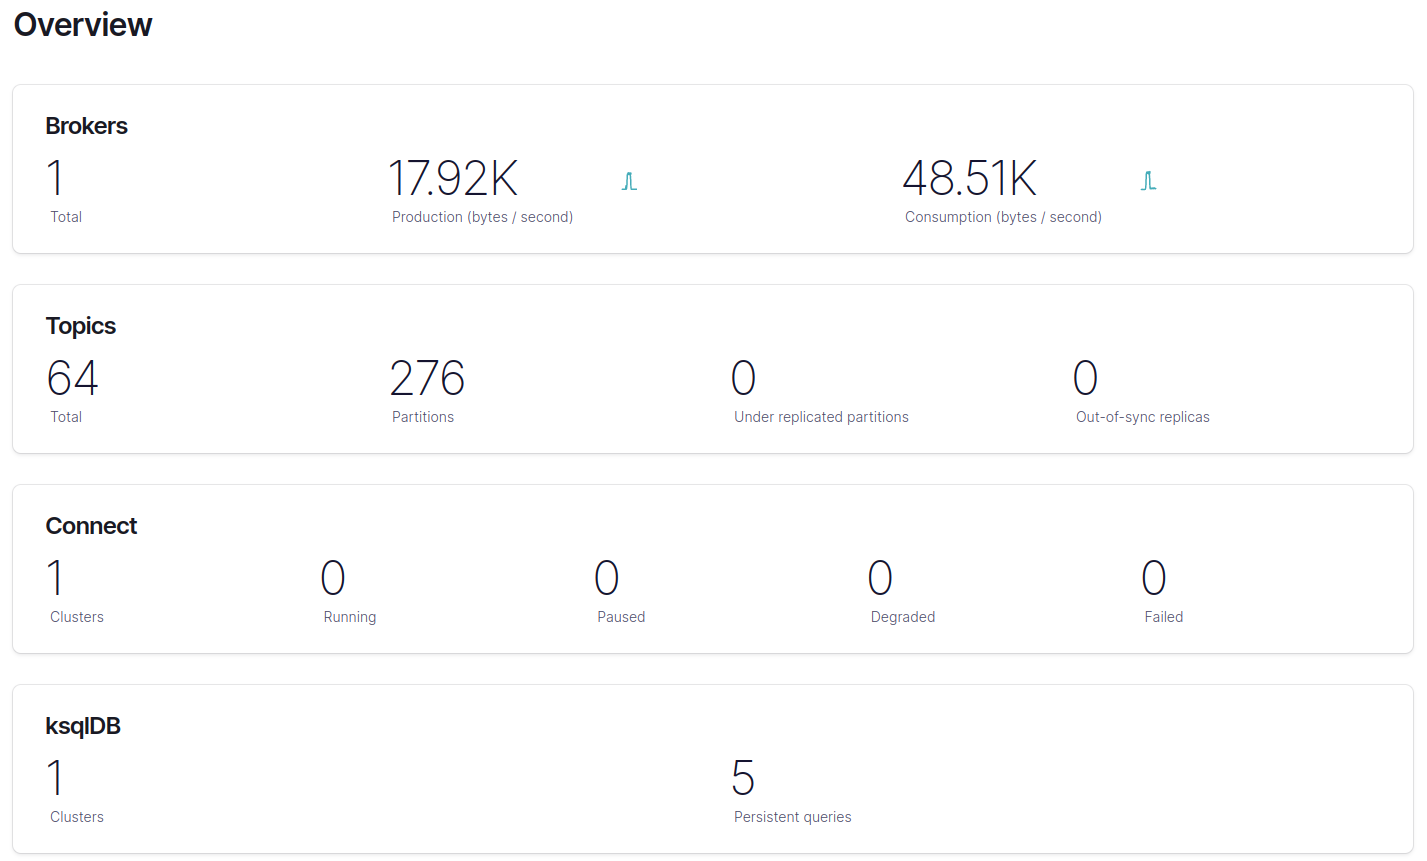
\includegraphics[scale=.3]{assets/appendices/overview.png}}
    \caption{Cluster overview  }
    \label{fig}
\end{figure}
* Shown number of topics include hidden internal topics on Cluster Overview
\section{The average end-to-end latency}
\begin{figure}[H]
    \centerline{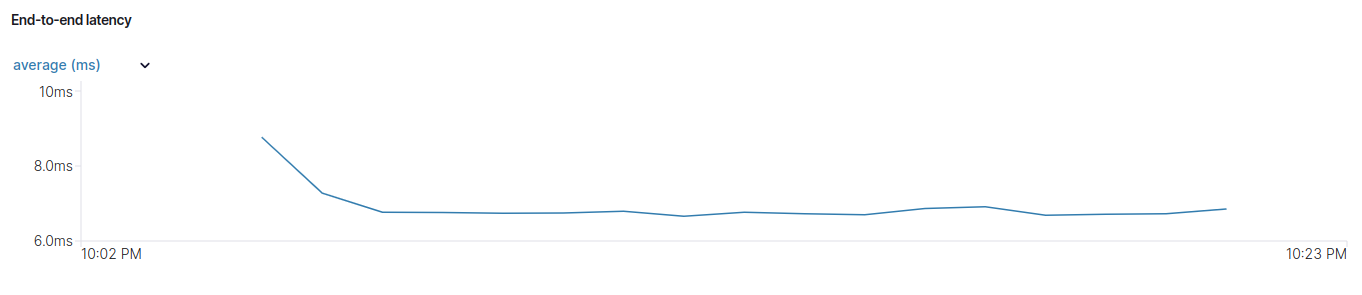
\includegraphics[scale=.4]{assets/appendices/average-end-to-end-latency.png}}
    \caption{The average end-to-end latency}
    \label{fig}
\end{figure}

\section{Throughput graph}
\begin{figure}[H]
    \centerline{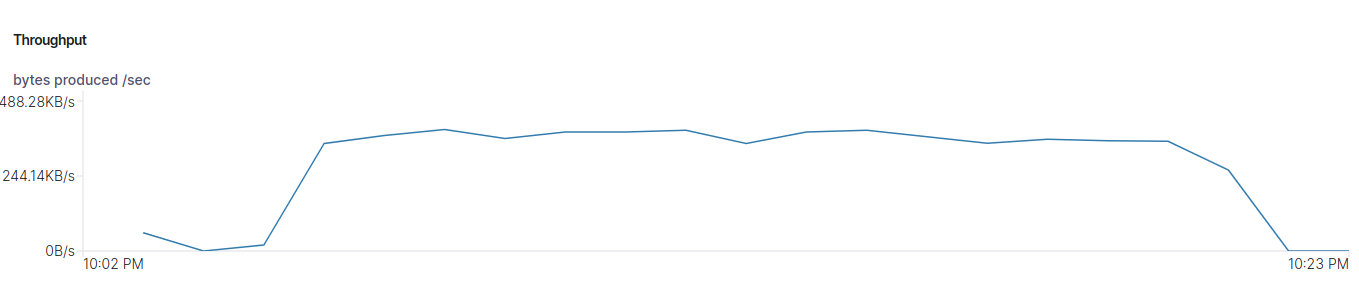
\includegraphics[scale=.4]{assets/appendices/throughput_graph.png}}
    \caption{Throughput graph}
    \label{fig}
\end{figure}

\section{Consumed throughput graph}
\begin{figure}[H]
    \centerline{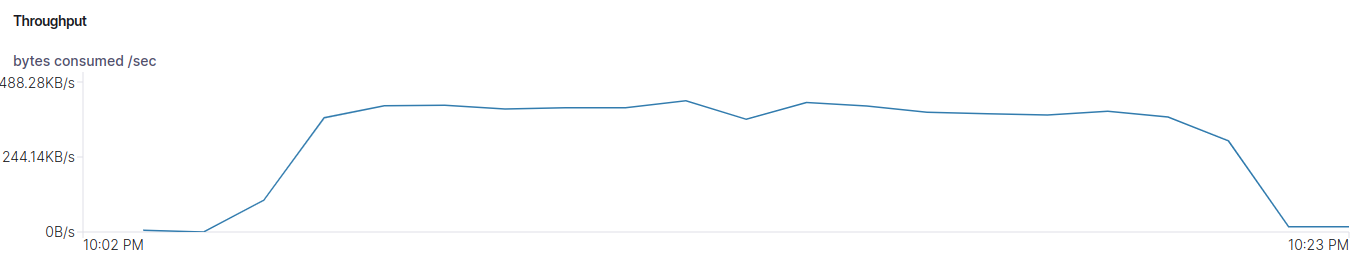
\includegraphics[scale=.4]{assets/appendices/throuhput-consumed.png}}
    \caption{Consumed throughput graph}
    \label{fig}
\end{figure}

\section{Topics}

\begin{figure}[H]
    \centerline{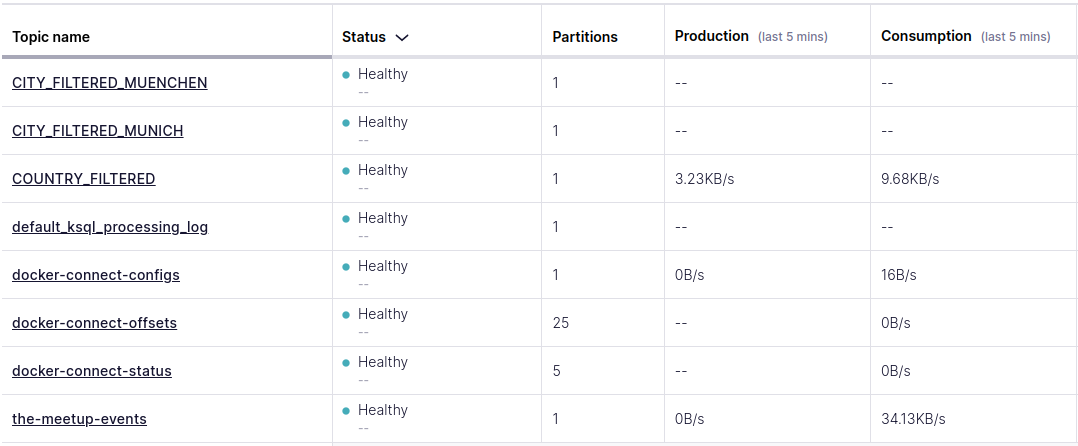
\includegraphics[scale=.4]{assets/appendices/topics-table.png}}
    \caption{Topics table}
    \label{fig}
\end{figure}

* Topics are automatically generated, topics which starts with `docker` and  `default` are internal topics.

\end{document}
\endinput
%%
%% End of file

